%-*- program: xelatex -*-        
%-*- program: biber -*-`        
%-*- program: xelatex -*-
\documentclass[11pt]{article}
\usepackage[margin=0.75in]{geometry}            % See geometry.pdf to learn the layout options. There are lots.
\geometry{letterpaper}  
\usepackage{amsmath,textcomp,amssymb,geometry,graphicx,enumerate,upquote,color}
\usepackage{hyperref}
\usepackage{breqn}
\usepackage{float}
\usepackage{tikz}
\usepackage{array}
\usepackage{float}
\usepackage{amsfonts}
\def\Session{Fall 2015}
\usepackage[english]{babel}
\title{Drawdown Project - Risk Contribution}
\author{Boying Gong, Xinyue Zhou}
\newenvironment{qparts}{\begin{enumerate}[{(}a{)}]}{\end{enumerate}}
\def\endproofmark{$\Box$}
\newenvironment{proof}{\par{\bf Proof}:}{\endproofmark\smallskip}
\begin{document}
\maketitle

\tableofcontents

\clearpage

\section{Empirical analysis using two asset class}

In this section, we present the empirical analysis of portfolio risk using two asset class, SPX (S\&P 500 Index) and RMZ (MSCI US REIT Index) in 60/40, 50/50, 40/60 allocation separately. For each portfolio, we calculate the risk contributins of each asset component for CED, ES, VaR and volatility. The four measures indicate similar risk of portfolios over time, but large differences when it comes to risk contributions. The variation of risk contributions for ES, VaR and volatility resemble each other under fixed asset allocation weights. For asset SPX, while the its contribution to ES, VaR and volatility reached its peak during 2010, the contribution of SPX maximized during 2014. Note that in the case of 40/60 asset allocation, SPX contributes to over 98\% of the total CED in 2014. 

\begin{figure}[H]
\centering
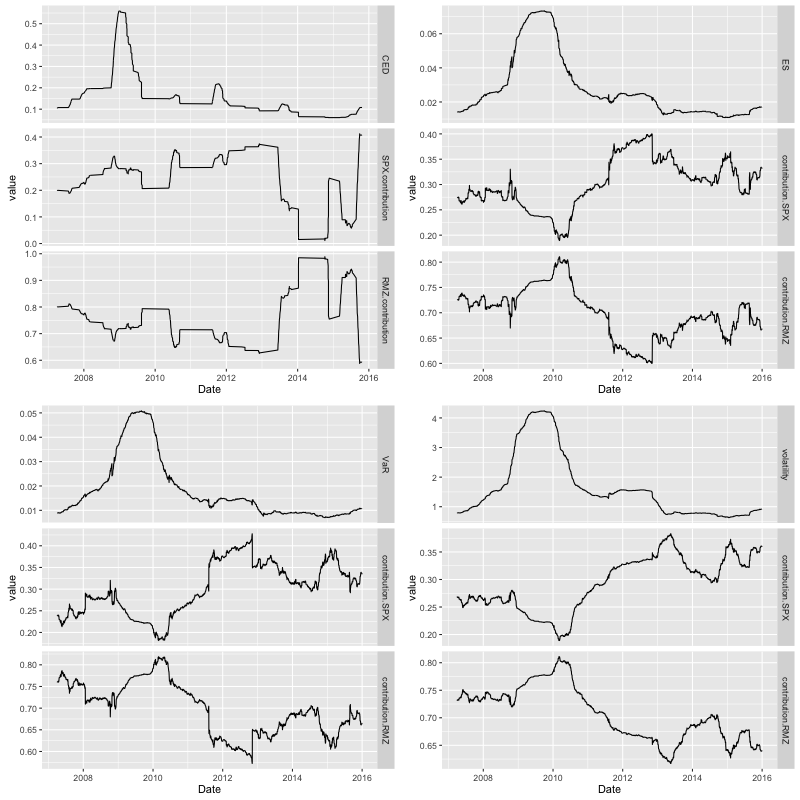
\includegraphics[width = 0.9\textwidth]{../figures/risk_contribution/SPX_RMZ_46}
\caption{3-month 1-year rolling risk contribution for CED, ES, VaR and volatility}
(portfolio is constructed using two asset classes (SPX and RMZ) in the balanced 40/60 allocation, probability level = 0.9)
\label{fig:risk_contribution_SPX_RMZ_46}
\end{figure}

\begin{figure}[H]
\centering
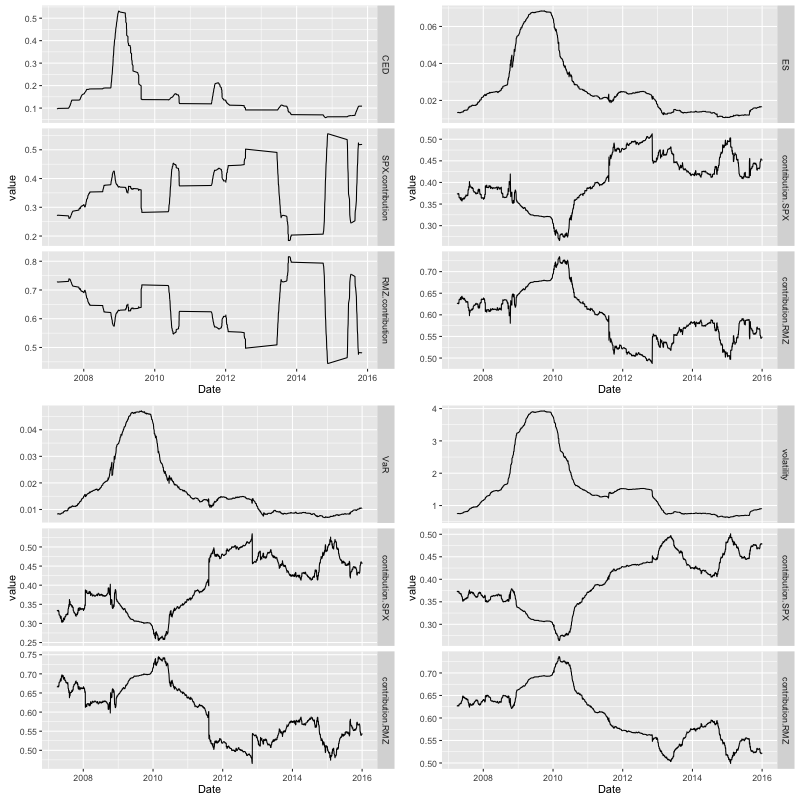
\includegraphics[width = 0.9\textwidth]{../figures/risk_contribution/SPX_RMZ_55}
\caption{3-month 1-year rolling risk contribution for CED, ES, VaR and volatility}
(portfolio is constructed using two asset classes (SPX and RMZ) in the balanced 50/50 allocation, probability level = 0.9)
\label{fig:risk_contribution_SPX_RMZ_55}
\end{figure}

\begin{figure}[H]
\centering
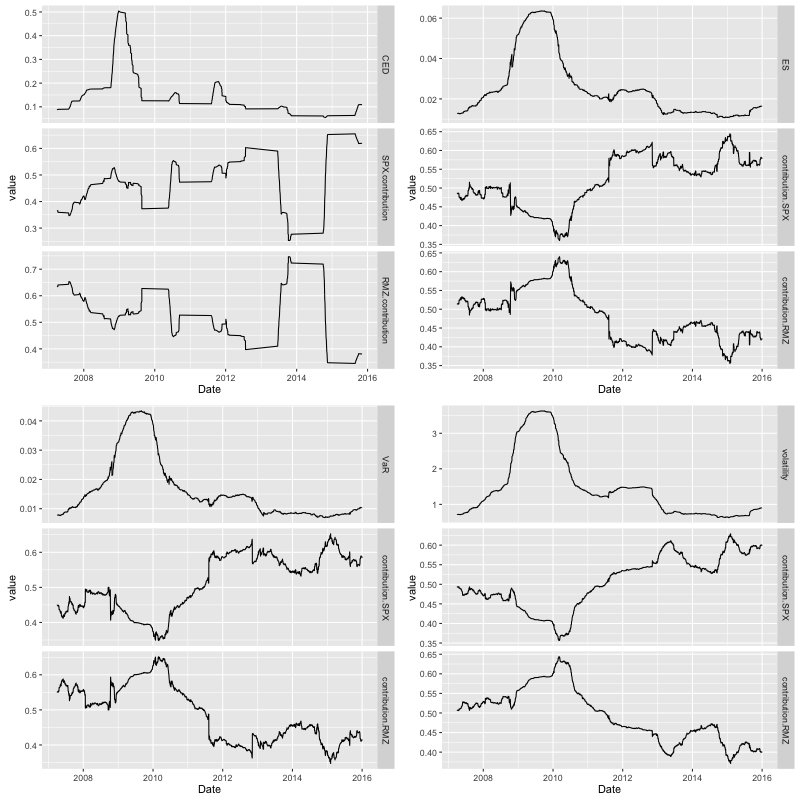
\includegraphics[width = 0.9\textwidth]{../figures/risk_contribution/SPX_RMZ_64}
\caption{3-month 1-year rolling risk contribution for CED, ES, VaR and volatility}
(portfolio is constructed using two asset classes (SPX and RMZ) in the balanced 60/40 allocation, probability level = 0.9)
\label{fig:risk_contribution_SPX_RMZ_64}
\end{figure}

% \begin{figure}[H]
% \centering
% 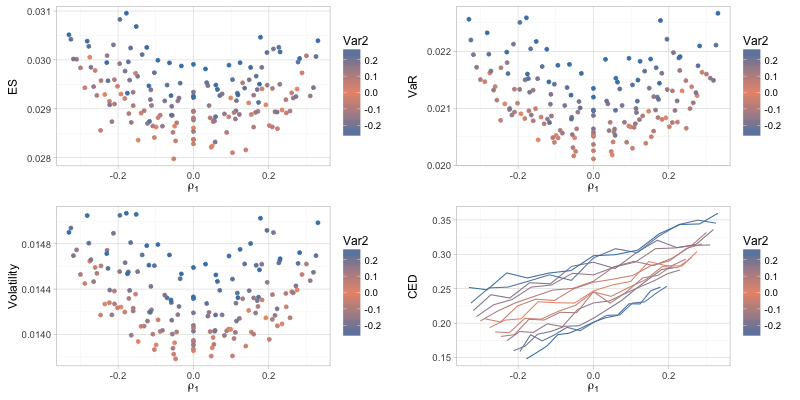
\includegraphics[width = 0.8\textwidth]{../figures/simulation/T_dist_MA2_risk_measures}
% \caption{MA(1): Relationship between serial correlation $\rho_1$ and risk measures}
% (Simulation path length: 63, $\epsilon_t \sim 0.01T(df = 4)$)
% \label{fig:T_dist_MA2_risk_measures}
% \end{figure}

% \begin{table}[H]
% \centering
% \begin{tabular}{|r |r r r r|}
% \hline
% & Mean & Sd & Skewness & Kurtosis \\
% \hline
% $\alpha = 0.05 $ & 0.0 & 0.029 & -0.003 & 0.088\\
% $\alpha = 0.08 $ & 0.0 & 0.013 & 0.001 & -0.033\\
% $\alpha = 0.11 $ & 0.0 & 0.011 & -0.000 & -0.001\\
% $\alpha = 0.14 $ & 0.0 & 0.011& -0.004 &  0.006\\
% $\alpha = 0.17 $ & 0.0 & 0.013 & -0.014 & -0.004\\
% $\alpha = 0.20 $ & 0.0 & 0.029 & 0.005 & 0.054\\
% \hline
% \end{tabular}
% \caption{Statistics of simulated return distribution of AR(1)+ GARCH(1,1)}
% \label{table:dist_garch_ar1_return}
% \end{table}

\end{document}













